\chapter{Asymmetrische Kryptosysteme}\label{chap:asymmetrische-kryptosysteme}

In den bisher angeschauten Verschlüsselungsverfahren haben wir festgestellt, dass derselbe Schlüssel zur Ver- und Entschlüsselung verwendet wird. Daher spricht man bei diesen Verfahren von \emph{symmetrischen} Verschlüsselungsmethoden. Zudem haben wir gesehen, dass diese entweder unsicher (Caesar, Vigenère) sind, wenn der Schlüssel einfach geknackt werden kann, oder unpraktikabel (\gls{OTP}), wenn der Schlüssel zuerst übertragen werden muss. Diffie \& Hellman kamen daher 1975 auf die Idee, \emph{asymmetrische} Verschlüsselungsverfahren zu erschaffen, welche nach einem anderen Prinzip funktionieren. Im Gegensatz zu symmetrischen Verfahren kann man bei asymmetrischen Verfahren \emph{nicht} von der verschlüsselten Nachricht auf den Schlüssel schliessen, da unterschiedliche Schlüssel zum Ver- und Entschlüsseln verwendet werden.

Die Grundidee hinter asymmetrischen Verschlüsselungsmethoden ist folgende:

Alice (\emoji{woman-technologist}) und Bob (\emoji{man-technologist}) möchten auf verschlüsselte Weise Nachrichten austauschen, die den Anforderungen an sichere Kryptosysteme genügen (siehe \cref{sec:intro}). Bei der asymmetrischen Verschlüsselung generieren sowohl Alice wie Bob jeweils ein Schlüsselpaar, einen sogenannten \textbf{öffentlichen Schlüssel} (\emoji{key}), der von allen Personen gesehen und verwendet werden kann, sowie einen \textbf{privaten Schlüssel} (\emoji{lock}), der nur im Besitz von Alice bzw. Bob ist. Wenn Alice eine Nachricht an Bob senden will, verwendet sie Bobs \emph{öffentlichen} Schlüssel, um die Nachricht zu verschlüsseln. Die Nachricht kann jedoch mit dem öffentlichen Schlüssel nicht entschlüsselt werden, es handelt sich hier sozusagen um eine \emph{Einweg}-Funktion. Stattdessen muss Bob seinen \emph{privaten} Schlüssel zur Entschlüsselung verwenden, also den Schlüssel, auf den \emph{nur} Bob Zugriff hat (siehe \cref{fig:public-key-encryption}). Dies funktioniert in den meisten Fällen auch in die andere Richtung: eine Nachricht, die mit Bobs privatem Schlüssel verschlüsselt worden ist, kann nur mit Bobs öffentlichem Schlüssel entschlüsselt werden. Die Schlüssel sind mathematisch so konstruiert, dass es beinahe unmöglich ist, vom öffentlichen Schlüssel auf den privaten Schlüssel zu schliessen.


Durch den Aufbau asymmetrischer Verschlüsselungsverfahren entfällt die Problematik der Übermittlung des Schlüssels: jede Person generiert ihr eigenes Schlüsselpaar und stellt einen öffentlichen Schlüssel zur Verfügung. Ein Nachteil hierbei ist, dass die Verschlüsselung häufig mathematisch und bezüglich Rechenleistung anspruchsvoller ist, was insbesondere problematisch sein kann bei längeren Nachrichten oder wenn die Antwortzeit minimal sein soll.

\begin{figure}[H]
	\centering
	\begin{tikzpicture}[node distance = 1cm and 2cm, data/.style={rectangle, rounded corners, text width=3cm, minimum width=3cm, minimum height=1cm, text centered, draw=ForestGreen, fill=ForestGreen!30},
			startstop/.style={rectangle, rounded corners, minimum height=1cm, minimum width=3cm, text width=2.5cm, text centered, draw=RoyalBlue, fill=RoyalBlue!30}]

		\footnotesize
		% Nodes
		\node (plaintext) [data] {\emoji{woman-technologist} Alice};
		\node (ciphertext) [data, right=of plaintext] {Verschlüsselter\\Text};
		\node (publickey) [startstop, above=of ciphertext] {\emoji{key} Öffentlicher Schlüssel\\von Bob};

		\node (decryptedtext) [data, below=of ciphertext] {Verschlüsselter\\Text};
		\node (privatekey) [startstop, below=of decryptedtext] {\emoji{lock} Privater Schlüssel\\ von Bob};
		\node (bob) [data, left=of decryptedtext] {\emoji{man-technologist} Bob};


		% Arrows
		\draw [->] (plaintext) -- (ciphertext);
		\draw [->] (ciphertext) -- (decryptedtext);
		\draw [->] (publickey) -- (ciphertext);
		\draw [->] (privatekey) -- (decryptedtext);
		\draw [->] (decryptedtext) -- (bob);

		\node at ($(plaintext.east)!0.5!(ciphertext.west)$) [above] {Klartext};
		\node at ($(publickey.south)!0.5!(ciphertext.north)$) [left] {Verschlüsselung};
		\node at ($(ciphertext.south)!0.5!(decryptedtext.north)$) [left] {Übertragung};
		\node at ($(privatekey.north)!0.5!(decryptedtext.south)$) [left] {Entschlüsselung};
		\node at ($(decryptedtext.west)!0.5!(bob.east)$) [above] {Klartext};
	\end{tikzpicture}
	\caption{Prinzip der Public-Key-Verschlüsselung}
	\label{fig:public-key-encryption}
\end{figure}

\section{\texorpdfstring{\acrshort{RSA}}{RSA}-Verfahren}
\label{subsec:rsa}

Das \acrfull{RSA}-Verfahren ist ein asymmetrisches Kryptosystem, das sowohl für die Verschlüsselung als auch für digitale Signaturen verwendet werden kann. Es basiert auf der Schwierigkeit, grosse Zahlen in ihre Primfaktoren zu zerlegen. Im Folgenden werden die Grundlagen des Verfahrens und ein einfaches Beispiel vorgestellt.

\begin{figure}[H]
	\centering
	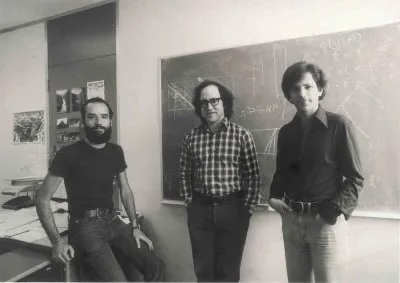
\includegraphics[width=0.7\linewidth]{Grundlagen_Info/03_Kryptologie/Figures/rsa.jpg}
	\caption{Ron Rivest, Adi Shamir und Leonard Adleman, die Erfinder des \gls{RSA}-Verfahrens}
	\label{fig:rsa}
\end{figure}


\begin{myprocedure}[\gls{RSA}-Verschlüsselungsverfahren]\label{myprocedure:RSA}
	Das \gls{RSA}-Verfahren besteht aus folgenden Schritten:
\begin{enumerate}
	\item \textbf{Schlüsselerzeugung:}
	      \begin{itemize}
		      \item Wählen Sie zwei (möglichst grosse) Primzahlen \( p \) und \( q \).
		      \item Berechnen Sie das \gls{RSA}-Modul \( n = p \cdot q \).
		      \item Berechnen Sie die Eulersche Funktion \( \varphi(n) = (p-1)(q-1) \).
		      \item Wählen Sie den \emph{Verschlüsselungsexponenten} \( e \), so dass dieser teilerfremd zu \( \varphi(n) \) und kleiner als $\varphi(n)$ ist. Dies bedeutet, dass der \gls{GGT} von $e$ und $\varphi(n)$ 1 ist ($\operatorname{ggT}(e, \varphi(n)) = 1$).
		      \item Berechnen Sie den \emph{Entschlüsselungsexponenten} \( d \), so dass \( (e \cdot d) \mod \varphi(n) = 1  \) (privater Schlüssel). Dies bedeutet, dass, wenn man $d$ mit $e$ multipliziert und dieses Produkt Modulo $\varphi(n)$ rechnet, man die Zahl 1 erhält.
		      \item Die Zahlen $p$, $q$ und $\varphi(n)$ werden nun nicht mehr benötigt und können gelöscht werden.
	      \end{itemize}
	\item \textbf{Verschlüsselung:}
	      \begin{itemize}
		      \item Der Absender verschlüsselt eine \textbf{Klartext-Nachricht} \( \mathbf{m} \) (als Zahl) mit dem \textbf{öffentlichen Schlüssel} \( \mathbf{(e, n)} \):
		            \[
			            c = \mathbf{m}^e \mod n
		            \]
		      \item Das Ergebnis \( c \) ist der Kryptotext.
	      \end{itemize}
	\item \textbf{Entschlüsselung:}
	      \begin{itemize}
		      \item Der Empfänger entschlüsselt die \textbf{verschlüsselte Nachricht} \( \mathbf{c} \) mit dem \textbf{privaten Schlüssel} \( \mathbf{(d, n)} \):
		            \[
			            \mathbf{m} = c^d \mod n
		            \]
		      \item Das Ergebnis \( \mathbf{m} \) ist die ursprüngliche Nachricht.
	      \end{itemize}
\end{enumerate}
\end{myprocedure}

\begin{myexample}
Um \gls{RSA} besser zu verstehen, rechnen wir ein einfaches Beispiel mit kleinen Zahlen durch:
\begin{enumerate}
	\item Wir wählen zwei (für diese Übung kleine) Primzahlen aus, \( p = 3 \) und \( q = 11 \). Daraus folgt:
	      \begin{align*}
		      n & = p \cdot q  \\
		        & = 3 \cdot 11 \\
		        & = 33
	      \end{align*}
	      \begin{align*}
		      \varphi(n) & = (p-1)(q-1) \\
		                 & = 2 \cdot 10 \\
		                 & = 20
	      \end{align*}
	\item Wir wählen \( e = 3 \), da \( \operatorname{ggT}(3, 20) = 1 \).
	\item Wir berechnen \( d \), so dass \( (e \cdot d) \mod \varphi(n) = 1  \) ergibt:
	      \[
		      (d \cdot 3) \mod 20 = 1  \quad \rightarrow \quad d = 7.
	      \]
	\item Der öffentliche Schlüssel ist \( (e, n) = (3, 33) \), der private Schlüssel \( (d, n) = (7, 33) \).
\end{enumerate}

\textbf{Verschlüsselung:} Die Nachricht sei der Klartext \texttt{Code}, welches wir darstellen durch die Position der Buchstaben im Alphabet \( m = 3, 15, 4, 5 \). Berechne für jeden Buchstaben (hier nur für \texttt{C}, also 3, gezeigt):
\begin{align*}
	c & = m^e \mod n  \\
	  & = 3^3 \mod 33 \\
	  & = 27 \mod 33  \\
	  & = 27.
\end{align*}


Der erste Buchstabe des Kryptotext wird also verschlüsselt als \( c = 27\).

\textbf{Entschlüsselung:}
\begin{align*}
	m & = c^d \mod n     \\
	  & = 27^{7} \mod 33 \\
	  & = 3
\end{align*}

Daraus ergibt sich \( m = 3 \), also die ursprüngliche Nachricht.
\end{myexample}


\begin{myexercise}\label{myexercise:rsa}
	Alice möchte eine Nachricht an Bob mit \gls{RSA} verschlüsseln. Bob wählt die Hilfs-Primzahlen \( p = 5 \) und \( q = 7 \). Generieren Sie den öffentlichen Schlüssel ($e, n$) und den privaten Schlüssel ($d, n$) von Bob, indem Sie folgende Schritte ausführen:
	\begin{enumerate}
		\item Berechnen Sie \( n \) und \( \varphi(n) \).
		\item Sie wählen $e$ und $d$ aus.
	\end{enumerate}

	Verschlüsseln Sie nun die Nachricht \( m = 9 \) mit dem öffentlichen Schlüssel \( (e, n) \).

	Entschlüsseln Sie danach die verschlüsselte Nachricht \( c \) wieder mit dem privaten Schlüssel \( (d, n) \).
	\begin{myanswer}
		\begin{enumerate}
			\item \( n = p \cdot q = 5 \cdot 7 = 35 \), \( \varphi(n) = (p-1)(q-1) = 4 \cdot 6 = 24 \).
			\item Für $e$ können wir beispielsweise 5 wählen, da 5 teilerfremd mit 24 ist.
			\item \( (5 \cdot d) \mod 24 = 1\). Dies finden wir beispielsweise mit \( d = 5 \).
			\item Verschlüsselung:
			      \begin{align*}
				      c & = m^e\mod n   \\
				        & = 9^5 \mod 35 \\
				        & = 4
			      \end{align*}.
			\item Entschlüsselung:
			      \begin{align*}
				      m & = c^d\mod n    \\
				        & =4^{5} \mod 35 \\
				        & = 9
			      \end{align*}
		\end{enumerate}
	\end{myanswer}
\end{myexercise}

\begin{myexercise}
	Ist die Wahl von \( p \) und \( q \) im obigen Beispiel sinnvoll? Begründen Sie Ihre Antwort.
	\begin{myanswer}
		Nein, die Wahl von \( p \) und \( q \) ist nicht sinnvoll, da beide Primzahlen zu klein sind. In der Praxis sollten \( p \) und \( q \) jeweils mindestens 2048 Bit lang sein, um eine ausreichende Sicherheit zu gewährleisten. Ansonsten kann es, wie im vorliegenden Beispiel, vorkommen, dass der private Schlüssel leicht durch Faktorisierung von \( n \) berechnet werden kann, oder dass der private Schlüssel sogar gleich dem öffentlichen Schlüssel ist (wie in diesem Beispiel, wo \( d = e = 5 \)).
	\end{myanswer}
\end{myexercise}

\begin{mychallenge}\label{mychallenge:rsa-pair}
 Erstellen Sie nun zu zweit jeweils ein Schlüsselpaar mit dem \gls{RSA}-Verfahren. Verwenden Sie dazu Primzahlen \( p \) und \( q \) mit jeweils mindestens 2 Ziffern. Tauschen Sie danach Ihre öffentlichen Schlüssel aus und verschlüsseln Sie eine Nachricht (eine Zahl) an Ihren Partner. Entschlüsseln Sie danach die Nachricht wieder.
 
 Eine Liste der ersten 1000 Primzahlen finden Sie hier: \url{https://en.wikipedia.org/wiki/List_of_prime_numbers}.
\end{mychallenge}

\begin{mychallenge}
Verwenden Sie Ihre RSA-Schlüssel aus \ref{mychallenge:rsa-pair}, um eine echte Nachricht als Zahl auszutauschen (ein Wort). Um ein Wort in Zahlen umzuwandeln (Buchstabe für Buchstabe) können Sie folgendes Python-Skript verwenden:
\begin{lstlisting}
def text_to_numbers(text):
	numbers = []
	for char in text.upper():
		if char.isalpha():  # Nur Buchstaben berücksichtigen
			numbers.append(ord(char) - ord('A') + 1)  # A=1, B=2, ..., Z=26
	return numbers

print(text_to_numbers("ABC"))  # Ausgabe: [1, 2, 3]
\end{lstlisting}
\end{mychallenge}

\begin{mychallenge}
	Wählen Sie zwei Primzahlen \( p \) und \( q \) mit jeweils mindestens 3 Ziffern. Generieren Sie den öffentlichen und privaten Schlüssel. Verschlüsseln Sie eine Nachricht Ihrer Wahl und entschlüsseln Sie diese wieder. Verwenden Sie Python, um die Berechnungen durchzuführen.

	Die Zahl $d$ kann in Python folgendermassen berechnet werden:

	Eine Liste der ersten 1000 Primzahlen finden Sie hier: \url{https://en.wikipedia.org/wiki/List_of_prime_numbers}
	\begin{lstlisting}
d = pow(e, -1, phi_n)
	\end{lstlisting}
	\begin{myanswer}
		Beispiel mit \( p = 101 \) und \( q = 113 \):
		\lstinputlisting{Grundlagen_Info/03_Kryptologie/Python package/encryption/rsa_simple.py}
	\end{myanswer}
\end{mychallenge}

\subsection{Digitale Signaturen mit \texorpdfstring{\acrshort{RSA}}{RSA}}
Neben der Verschlüsselung von Nachrichten kann das \gls{RSA}-Verfahren auch zur Erstellung digitaler Signaturen verwendet werden. Digitale Signaturen dienen dazu, die Authentizität und Integrität einer Nachricht zu gewährleisten. Hierbei wird die Nachricht mit dem privaten Schlüssel des Absenders signiert, sodass der Empfänger die Signatur mit dem öffentlichen Schlüssel des Absenders überprüfen kann.

\begin{myprocedure}[Digitale Signaturen mit \gls{RSA}]
	Die Erstellung und Überprüfung digitaler Signaturen mit dem \gls{RSA}-Verfahren erfolgt in folgenden Schritten:
\begin{enumerate}
	\item \textbf{Signaturerstellung:}
	      \begin{itemize}
		      \item Der Absender erstellt eine \textbf{Nachricht} \( \mathbf{m} \).
		      \item Er berechnet den \textbf{Hashwert} \( H(m) \) der Nachricht \( m \) mithilfe einer kryptographischen Hashfunktion (z.B. SHA-256).
		      \item Der Absender signiert den Hashwert mit seinem \textbf{privaten Schlüssel} \( \mathbf{(d, n)} \):
		            \[
			            s = H(m)^d \mod n
		            \]
		      \item Das Ergebnis \( s \) ist die digitale Signatur.
	      \end{itemize}
	\item \textbf{Signaturüberprüfung:}
	      \begin{itemize}
		      \item Der Empfänger erhält die Nachricht \( m \) und die Signatur \( s \).
		      \item Er berechnet den Hashwert \( H(m) \) der empfangenen Nachricht \( m \).
		      \item Der Empfänger überprüft die Signatur mit dem \textbf{öffentlichen Schlüssel} \( \mathbf{(e, n)} \) des Absenders:
		            \[
			            H'(m) = s^e \mod n
		            \]
		      \item Wenn \( H'(m) = H(m) \), ist die Signatur gültig, andernfalls ist sie ungültig.
	      \end{itemize}
\end{enumerate}
\end{myprocedure}

\begin{myexample}
	Angenommen, Alice möchte eine Nachricht \( m = 42 \) signieren. Sie verwendet ihren privaten Schlüssel \( (d, n) = (9677, 12317) \) und den öffentlichen Schlüssel \( (e, n) = (5, 12317) \).

	\textbf{Signaturerstellung:}
	\begin{align*}
		s & = H(m)^d \mod n \\
		  & = 42^{9677} \mod 12317 \\
		  & = 161
	\end{align*}

	Die digitale Signatur ist also \( s = 161 \).

	\textbf{Signaturüberprüfung:}
	\begin{align*}
		H'(m) & = s^e \mod n \\
		      & = 161^5 \mod 12317 \\
		      & = 42
	\end{align*}

	Da \( H'(m) = H(m) \), ist die Signatur gültig.
\end{myexample}

\begin{myexercise}
	Alice möchte die Nachricht \( m = 15 \) signieren. Ihr privater Schlüssel ist \( (d, n) = (7, 33) \) und ihr öffentlicher Schlüssel ist \( (e, n) = (3, 33) \).

	Erstellen Sie die digitale Signatur \( s \) für die Nachricht \( m \).

	Überprüfen Sie danach die Signatur mit dem öffentlichen Schlüssel.
	\begin{myanswer}
		\textbf{Signaturerstellung:}
		\begin{align*}
			s & = H(m)^d \mod n \\
			  & = 15^{7} \mod 33 \\
			  & = 27
		\end{align*}

		Die digitale Signatur ist also \( s = 27 \).

		\textbf{Signaturüberprüfung:}
		\begin{align*}
			H'(m) & = s^e \mod n \\
			      & = 27^3 \mod 33 \\
			      & = 15
		\end{align*}

		Da \( H'(m) = H(m) \), ist die Signatur gültig.
	\end{myanswer}
\end{myexercise}